\chapter{Experimental results}
\indent
	PSNR on testing set is \textbf{25.79928}. \\
	Experiments of this chapter are done with setup below: 
	\begin{itemize}
		\item Seed: 42.
		\item Batch size: 64.
		\item Number of epochs and iterations: 100 / 600.
		\item Learning rate: $2 \times 10^{-3}$.
		\item Optimizer: \code{Adam} with betas (0.9, 0.999).
		\item RNN hidden size: 256.
		\item Number of hidden layers: 2 (predictor) / 1 (prior).
		\item RNN input and output size: 64 / 128.
	\end{itemize} 

\section{Video prediction on testing set}
	\begin{figure}[H]
		\centering
		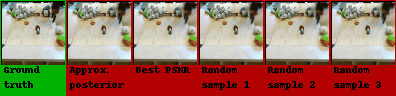
\includegraphics[scale=0.9]{img/test_pred-2.png}
		\caption{Samples from testing set (only 3rd frame is displayed here, details are in Appendix \ref{more-results}).}
		\label{test-prediction}
	\end{figure}

\section{KL loss and PSNR curves}
	From Figures \ref{result-mono} and \ref{result-cyc}, 
	we can see that I set the teacher-forcing ratio to fixed 1 during entire training, 
	and training loss decreases smoothly and PSNR increases fast under both monotonic and cyclical modes. 
	The unstable PSNR is partially due to the validation PSNR is tested each 5 epochs, 
	if we test it each epoch, the curve will be much more smooth. \\
	From my experiments, results of two modes seem similar, both for loss and PSNR.
	Also, the testing PSNR is similar to best validation PSNR, and even higher, i.e., 
	testing PSNR is \textbf{25.79928}, best validation PSNR for monotonic mode is \textbf{25.73145}, 
	and best validation PSNR for cyclical mode is \textbf{25.76462}.
	Exposure bias seems not occur during training with fixed teacher-forcing ratio 1.
	
	\begin{figure}[H]
		\centering
		\begin{subfigure}
			\centering
			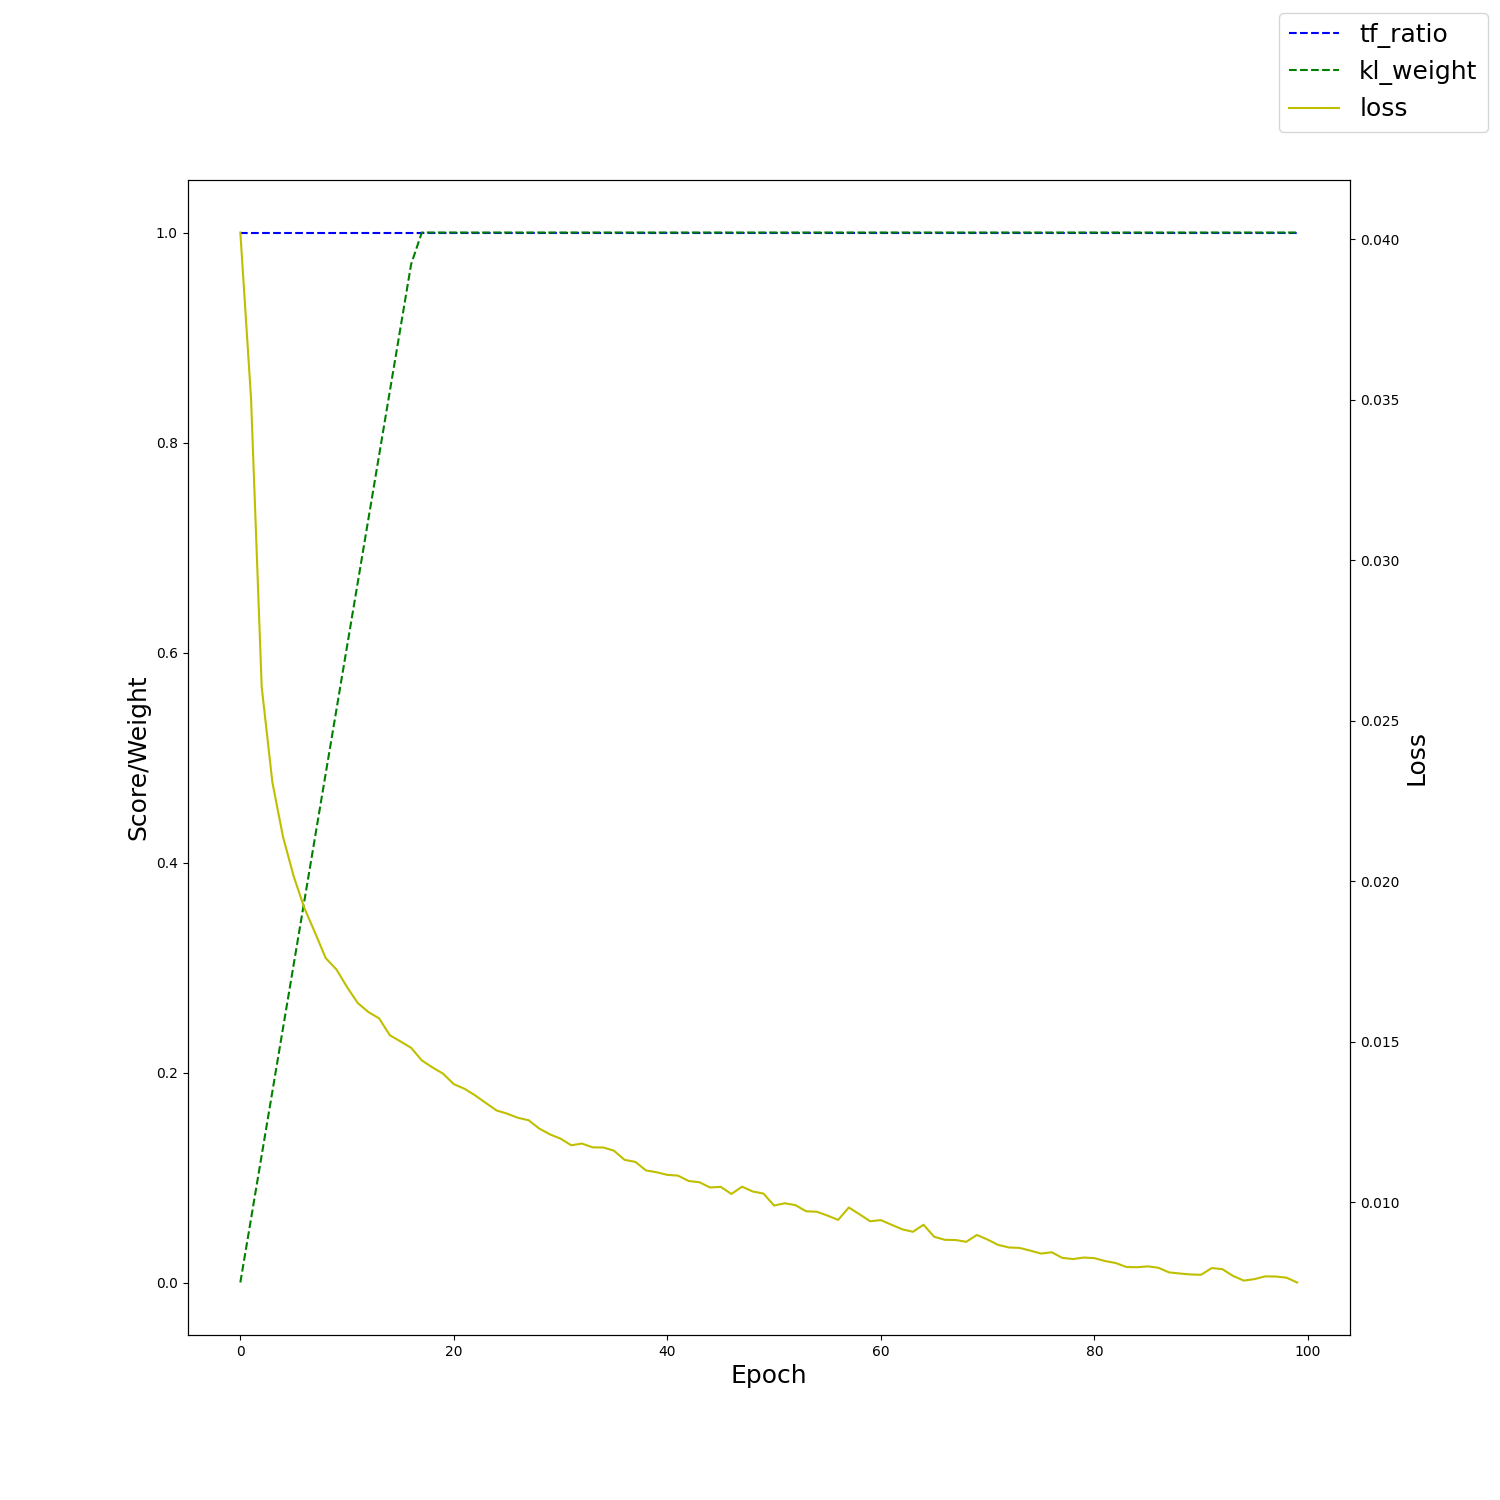
\includegraphics[width=0.45\textwidth]{img/loss_mono.png}
			\label{loss-mono}
		\end{subfigure}
		\hfill
		\begin{subfigure}
			\centering
			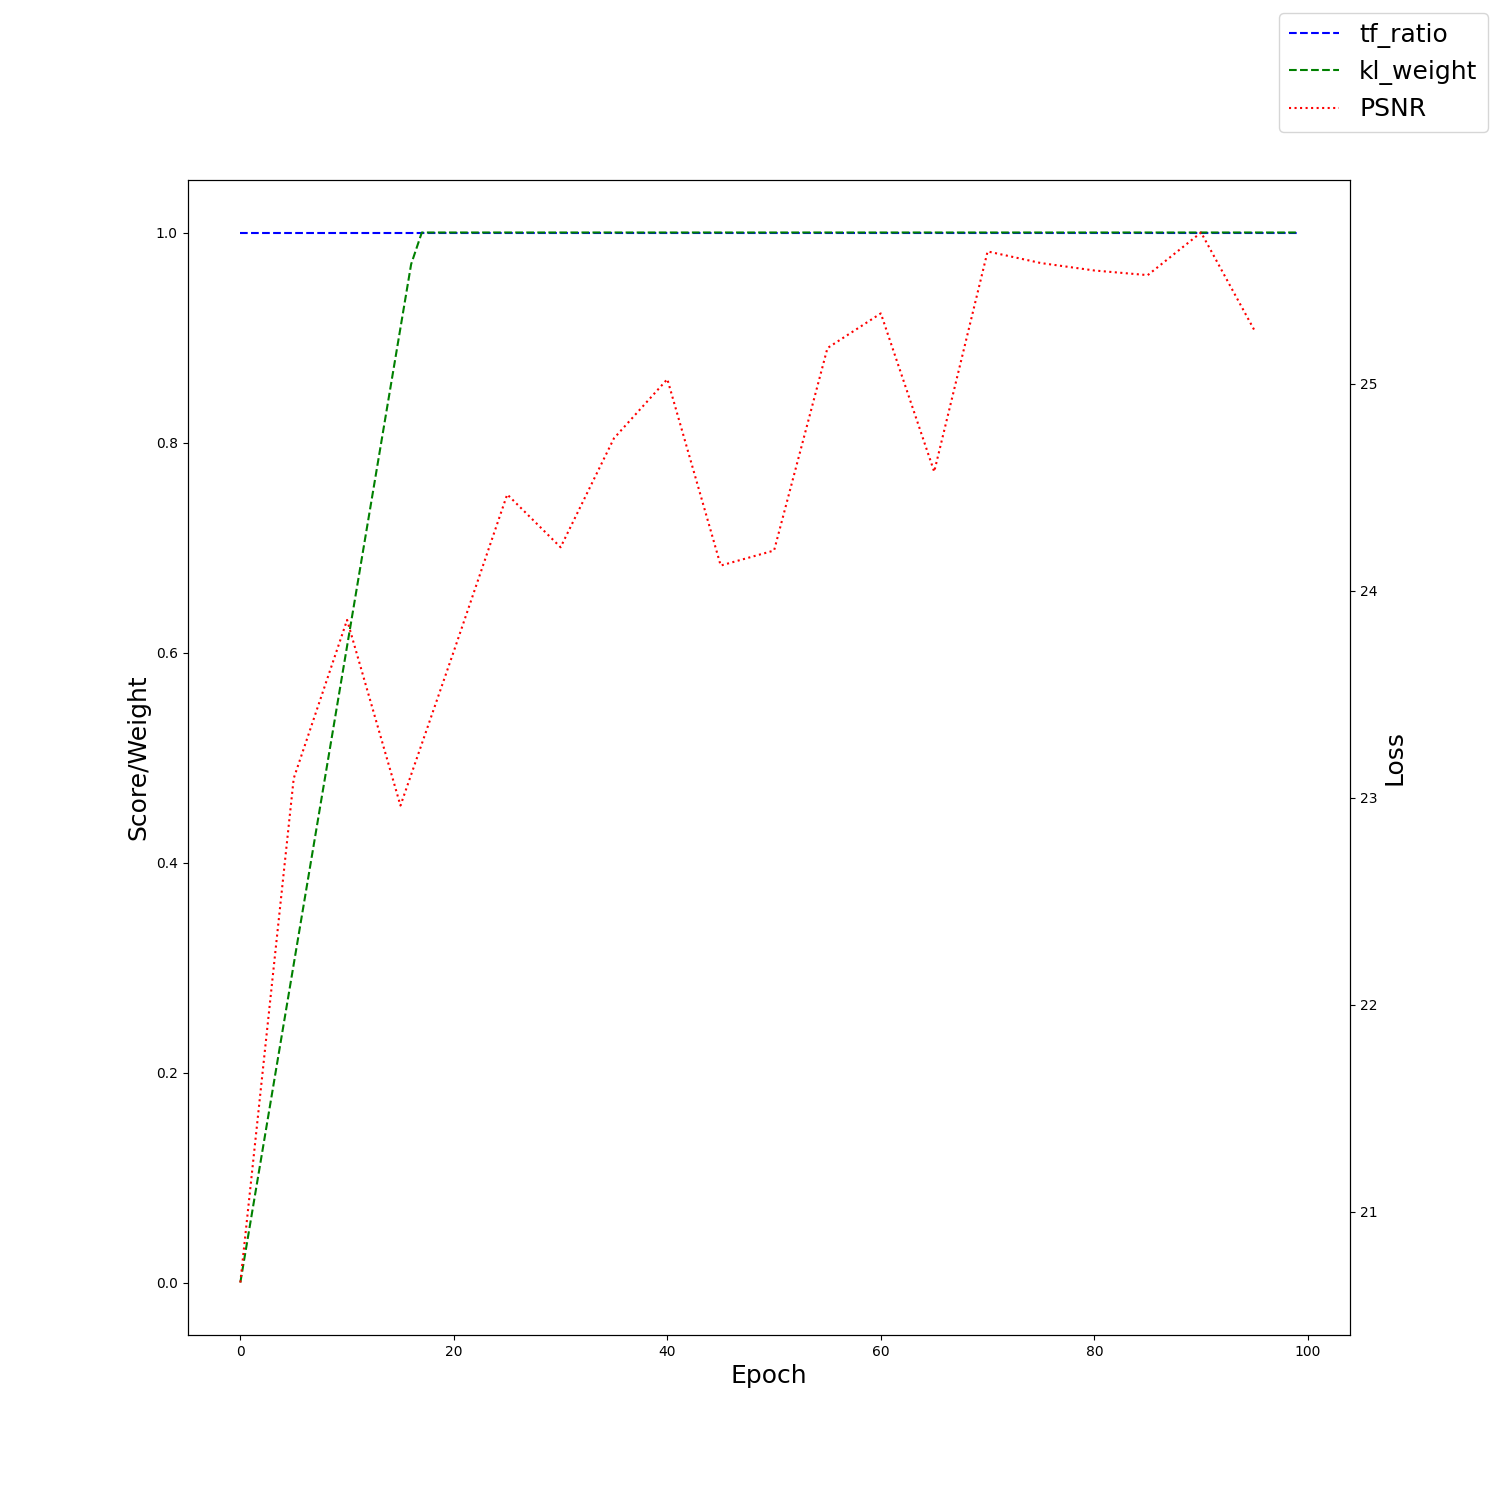
\includegraphics[width=0.45\textwidth]{img/psnr_mono.png}
			\label{psnr-mono}
		\end{subfigure}
		\hfill
		\caption{KL loss and PSNR of \textbf{monotonic} KL annealing mode.}
		\label{result-mono}
	\end{figure}

	\begin{figure}[H]
		\centering
		\begin{subfigure}
			\centering
			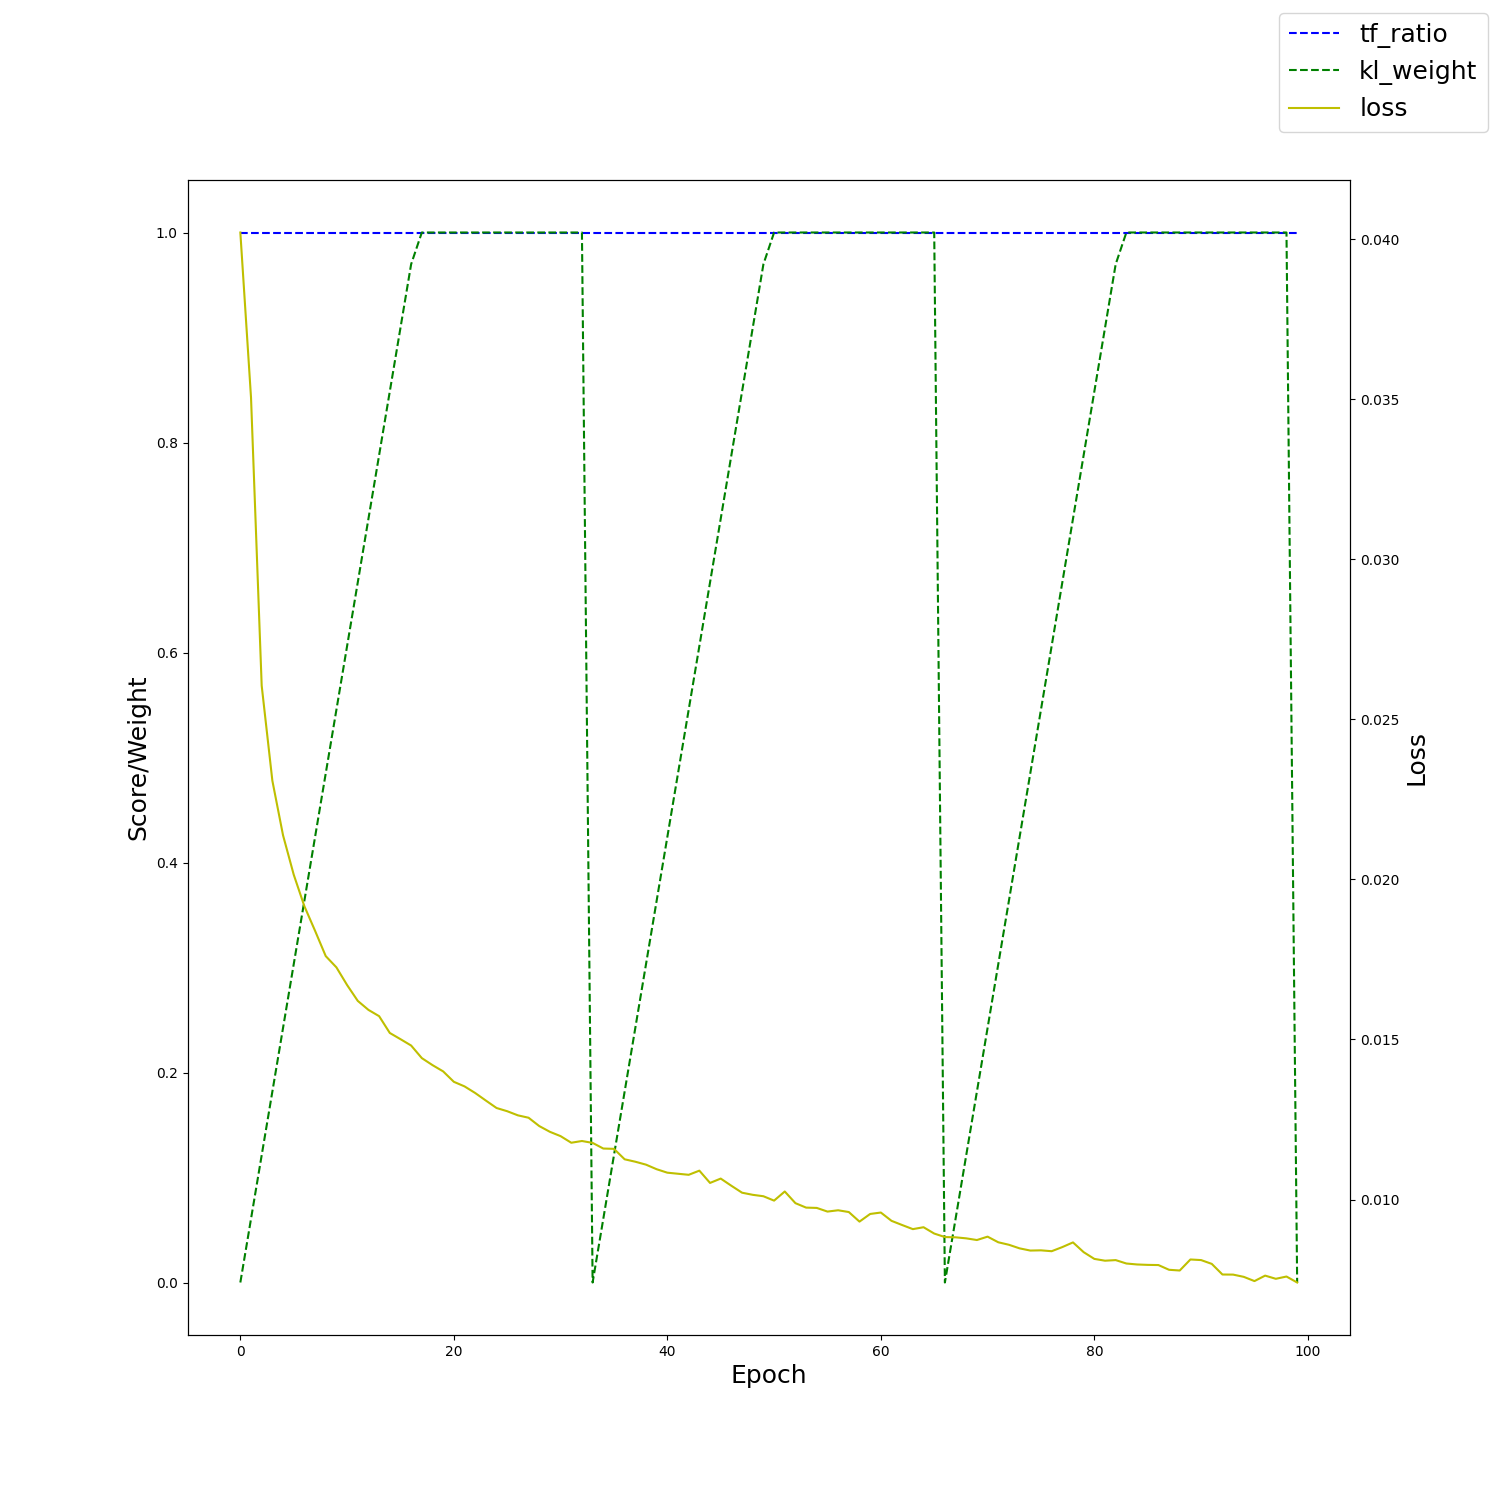
\includegraphics[width=0.45\textwidth]{img/loss_cyc.png}
			\label{loss-cyc}
		\end{subfigure}
		\hfill
		\begin{subfigure}
			\centering
			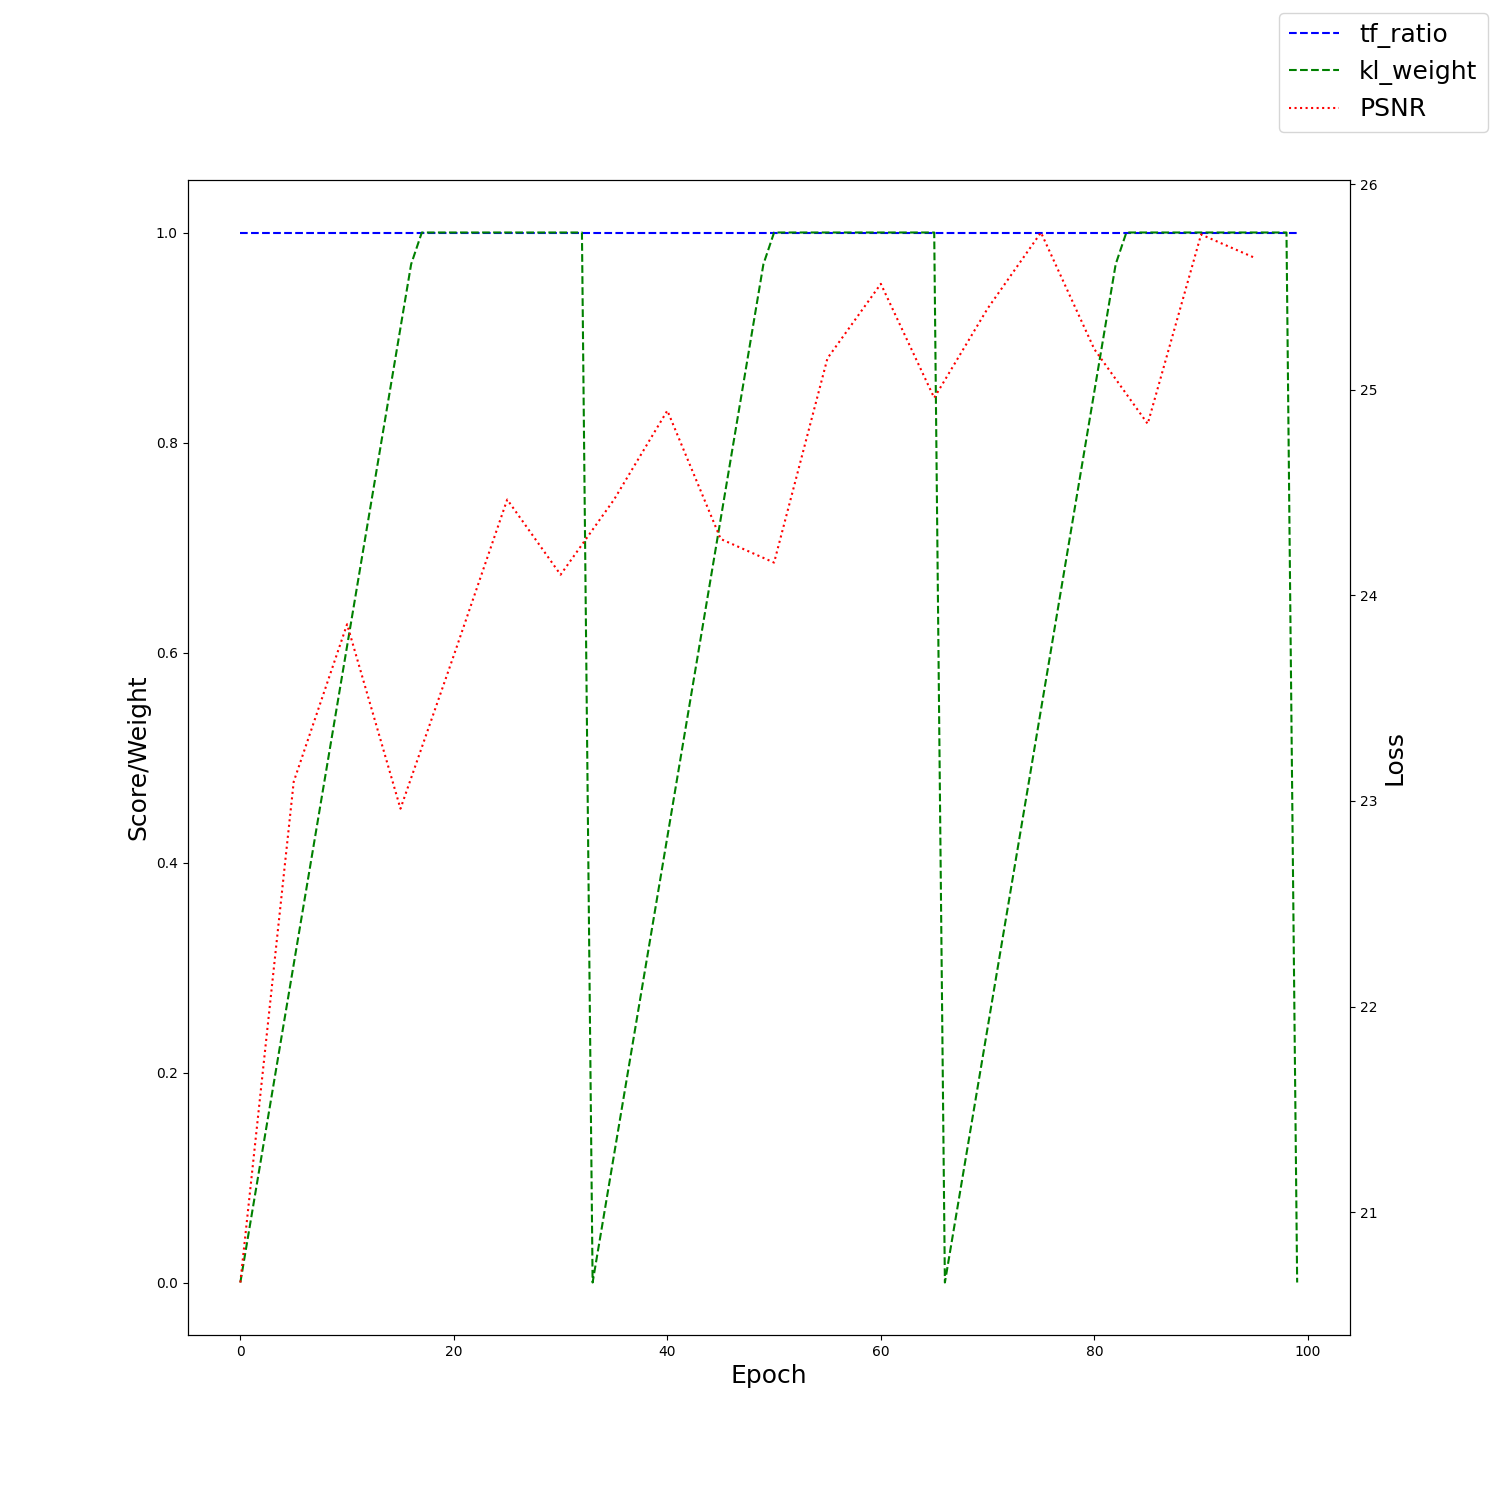
\includegraphics[width=0.45\textwidth]{img/psnr_cyc.png}
			\label{psnr-cyc}
		\end{subfigure}
		\hfill
		\caption{KL loss and PSNR of \textbf{cyclical} KL annealing mode.}
		\label{result-cyc}
	\end{figure}
